\chapter{Brief description of PAD}\label{s:pad}

\section{PAD is }

Problem Analysis Diagram (PAD) is to describe the logical structure of
the program by the two dimensional tree.
%
PAD is suitable for structured programing, like Fortran.




\section{Elements in PAD}

In PAD, one box shows one process or one sentence in Fortran, and
only three basic structure is allowed; sequence, conditional branch, and iteration.

\subsection{Sequence}

%
Simple sequence of sentence is shown as listed box in same vertical line
from top to bottom
(\autoref{f:pad_sequence}).
%
Subroutine call is shown as \autoref{f:pad_call}.


\begin{figure}[htbp]
\begin{minipage}{.49\textwidth}
\center
 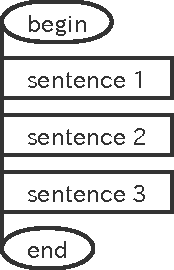
\includegraphics[scale=0.7]{figs/pad_sequence.pdf}
\end{minipage}
\begin{minipage}{.49\textwidth}
\begin{LstF90}[numbers=none]
 sentence 1
 sentence 2
 sentence 3
\end{LstF90}
\end{minipage}
\caption{elements of PAD: sequence}
\label{f:pad_sequence}
\end{figure}


\begin{figure}[htbp]
\begin{minipage}{.49\textwidth}
 \center
  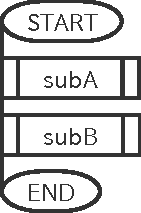
\includegraphics[scale=0.7]{figs/pad_routinecall.pdf}
\end{minipage}
\begin{minipage}{.49\textwidth}
\begin{LstF90}[numbers=none]
 call subA()
 call subB()
\end{LstF90}
\end{minipage}
 \caption{elements of PAD: subroutine call}
 \label{f:pad_call}
\end{figure}

\subsection{Conditional branch}

Conditional branch and selection are shown in the same manner.
\autoref{f:pad_if} shows the IF-THEN-ELSE type branch, and
\autoref{f:pad_case} shows the CASE type branch.

\begin{figure}[htbp]
\begin{minipage}{.49\textwidth}
 \center
  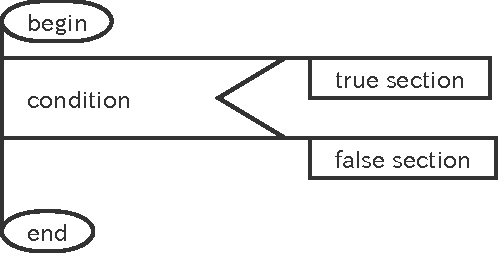
\includegraphics[scale=0.7]{figs/pad_ifelse.pdf}
\end{minipage}
\begin{minipage}{.49\textwidth}
\begin{LstF90}[numbers=none]
 if ( condition ) then
   true section
 else
   false section
 end if
\end{LstF90}
\end{minipage}
\caption{elements of PAD: IF-THEN-ELSE}
\label{f:pad_if}
\end{figure}

\begin{figure}[htbp]
\begin{minipage}{.6\textwidth}
 \center
  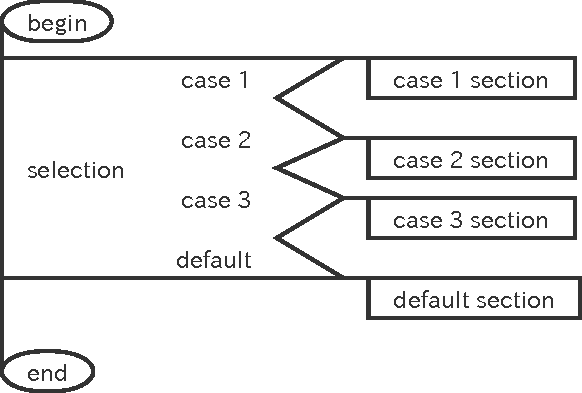
\includegraphics[scale=0.7]{figs/pad_selection.pdf}
\end{minipage}
\begin{minipage}{.4\textwidth}
\begin{LstF90}[numbers=none]
 select case ( selection )
 case (case1)
   case1 section
 case (case2)
   case2 section
 case (case3)
   case3 section
 case default
   default section
 end case
\end{LstF90}
\end{minipage}
\caption{elements of PAD: CASE Selection}
\label{f:pad_case}
\end{figure}

\subsection{Iteration}

Iteration is shown as \autoref{f:pad_iteration}.

\begin{figure}[htbp]
\begin{minipage}{.49\textwidth}
 \center
  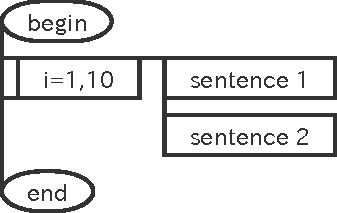
\includegraphics[scale=0.7]{figs/pad_iteration.pdf}
\end{minipage}
\begin{minipage}{.49\textwidth}
\begin{LstF90}[numbers=none]
 do i=1, 10
   sentence 1
   sentence 2
 end do
\end{LstF90}
\end{minipage}
\caption{elements of PAD: Iteration}
\label{f:pad_iteration}
\end{figure}


\subsection{Hierarchy}

Hierarchy in program is expressed as connection of boxes in right
direction.
%
So width of the PAD means complexity of the program and height means the
size of the program.
%
\autoref{f:pad_hierarcy} shows the example of hierarcy in PAD.
%
The first half shows combination of IF-THEN-ELSE clause and DO-loop, the
latter half shows usual double Do-loop.

\begin{figure}[htbp]
\begin{minipage}{.7\textwidth}
 \center
  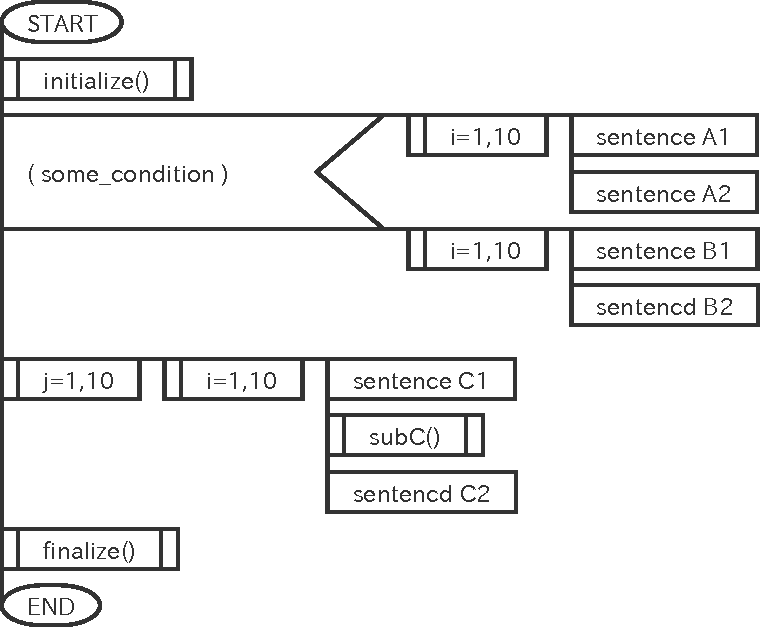
\includegraphics[scale=0.7]{figs/pad_hierarcy.pdf}
\end{minipage}
\begin{minipage}{.29\textwidth}
\begin{LstF90}[numbers=none]
 call initialize()

 if ( some_condition ) then
   do i=1,10
     sentence A1
     sentence A2
   end do
 else
   do i=1,10
     sentence B1
     sentence B2
   end do
 end if

 do j=1,10
   do i=1,10
     sentence C1
     call subC()
     sentence C2
   end do
 end do

 call finalize()
\end{LstF90}
\end{minipage}
\caption{Example of hierarcy in PAD}
\label{f:pad_hierarcy}
\end{figure}
